\documentclass[12pt,a4paper]{article}
\usepackage[utf8]{inputenc}
\usepackage{amsmath}
\usepackage{amsfonts}
\usepackage{amssymb}
\usepackage{graphicx}
\usepackage{hyperref}
\usepackage[margin=0.5in]{geometry}

\graphicspath{ {./images/} }
\author{Oleg Loshkin}
\title{Simple Online FPS}

\hypersetup{
    colorlinks=true,
    linkcolor=blue,
    filecolor=magenta,      
    urlcolor=cyan,
}

\begin{document}

\maketitle

\section{Introduction}
This game is the result of the \textbf{SAE's repeat session for the GPR5100 Game Networking module}. \textbf{The aim of this project was to make a simple but functional online game} using Unity and a networking technology of our choice.

\section{Technologies used}
\begin{itemize}
\item \textbf{Unity 2018.4.9f1:}\\
Latest available LTS version of Unity available at the time the project had started.
\item \textbf{Photon Bolt:}\\
High level game networking API for Unity. \textbf{The API provides some features that match perfectly the requirements of an online FPS}, namely lag compensating hitboxes and raycasting which negates the need to implement this complex feature manually.
\item \textbf{Github:}\\
Github was used for versioning. \textbf{The project's repository is available \href{https://github.com/LoshkinOleg/NetworkingRattrapage}{here}} .\\
The repository was temporarely split between two branches mid project to explore a possible migration to Photon Pun. This idea was abandonned and game was implemented using Photon Bolt.
\end{itemize}

\section{Gameplay}
\begin{center}
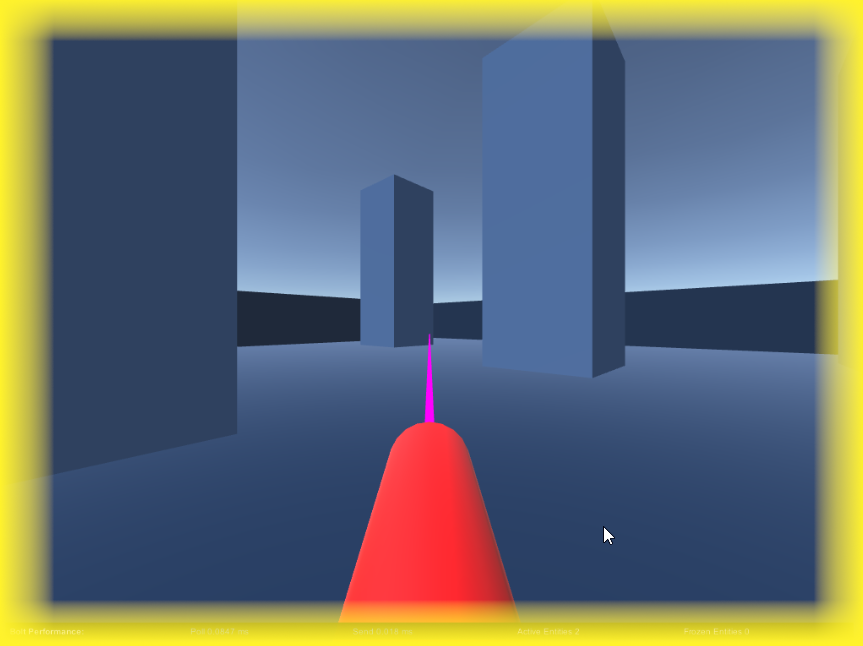
\includegraphics[scale=0.75]{gameplay}
\end{center}
\begin{itemize}
\item \textbf{The Lobby:}\\
The player can either \textbf{create a new game session} and name it \textbf{or join a random game session currently in progress}. Upon the creation of a session, the host joins it as a listen server.\\
Note that the session's name is currently unused as no list of sessions is visible anywhere, that sessions cannot be password protected and the number of maximum players per session cannot be established.
\item \textbf{The Arena:}\\
The arena is a \textbf{square area surrounded by walls and dotted with pillars that server as cover}. \textbf{Spawn points are located on the outer periphery of the arena close to the pillars}.
\item \textbf{The Controls:}\\
Players can \textbf{shoot with Left Mouse Button}, \textbf{look around horizontally only using the mouse} and \textbf{move around using WASD keys}.
\item \textbf{The Fight:}\\
\textbf{A 2 second cooldown is enforced between each shot} a player takes. \textbf{A player can take two hits from an adversary before dying}. No ways to regenerate health exist. \textbf{Upon death, the player respawns at the spawn point furthest away from the average position of all other players}.
\newpage
\item \textbf{The Feedbacks:}\\
\begin{itemize}
\item A \textbf{shooting sound} is played upon any shot.
\item A \textbf{reloading sound} is played just before the end of the shooting cooldown and \textbf{the sound's end indicates the end of the cooldown}. Only the local player hears this sound.
\item \textbf{Getting hit} triggers a \textbf{grunting} sound from the player. Only the player being hit hears this sound.
\item \textbf{Upon landing a shot} on a player, \textbf{a ringing sound is played} for every player except the one being hit.
\item Upon \textbf{being hit once}, the player's \textbf{screen edges turn yellow}. \textbf{Being hit a second time} turns the \textbf{edges turn red}. A third hit kills the player and the health indicating overlay resets.
\end{itemize}
\end{itemize}

\section{Movement}
The movement in the game is \textbf{client authoritative} and uses \textbf{interpolation}. It is implemented using \textbf{Photon Bolt's Transform State and Commands}. While using RigidBodies is impossible in conjunction with Photon Bolt, Unity's "Character Controller" component has provided a good replacement for movement and collisions.\\\\
Client authoritativity not being ideal in online FPS games, a server authoritative movement was originally planned. However, after much efforts trying to make it work, Photon Bolt's rollback and lack of documentation of it's inner workings has made this idea too difficult to execute.

\section{Hitscanning}
Implementation of hitscanning was surprisingly easy using \textbf{Photon Bolt's Hitboxes and it's BoltNetwork.RaycastAll() method}. The only caveats that had to be worked around was the inability to filter the targets and the fact that the raycast does not interact with non-Bolt game objects like walls.
\newpage

\section{Lobby}
\begin{center}
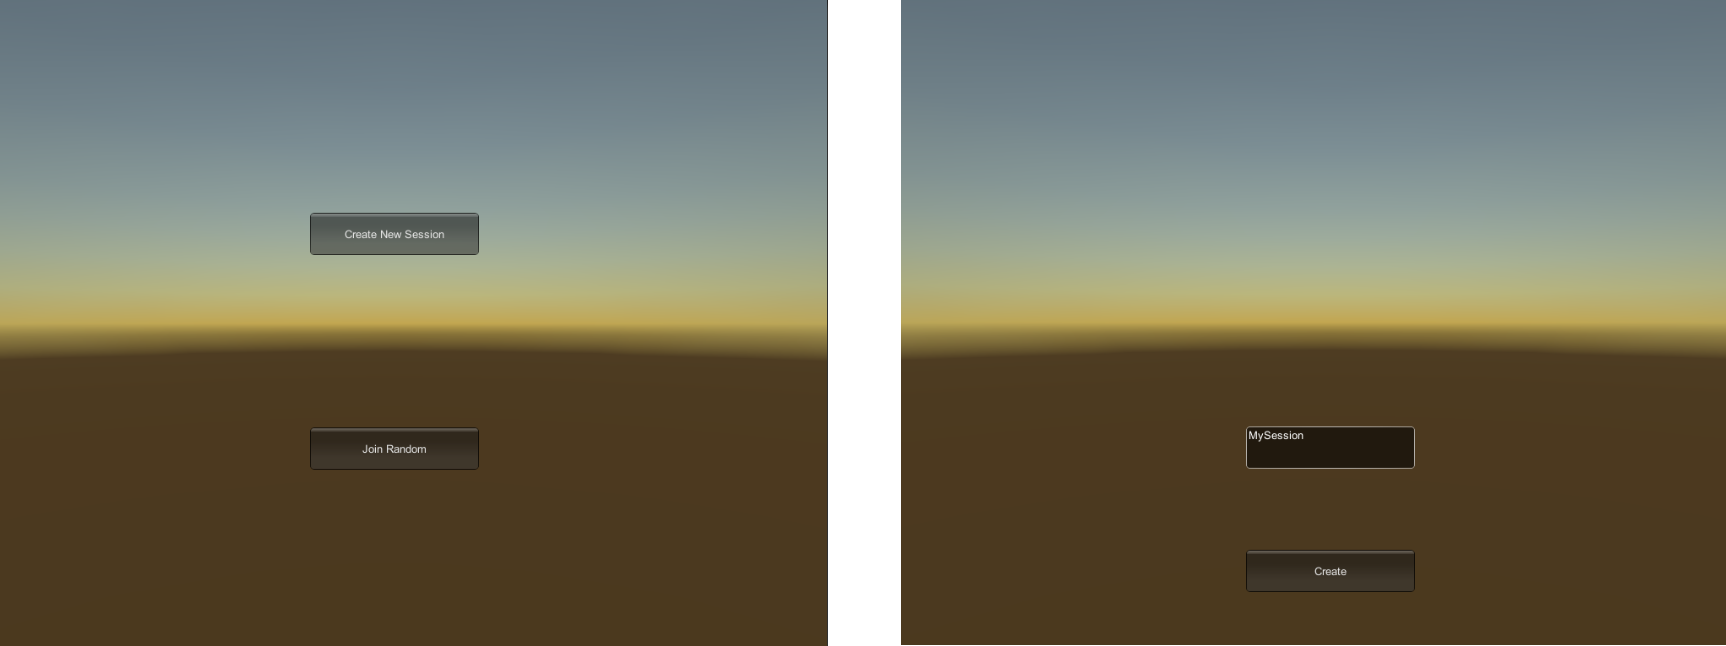
\includegraphics[scale=0.4]{lobby}
\end{center}
The lobby is comprised of \textbf{two tabs}: a main one with two buttons for \textbf{creating a new session or to join a random one}, and \textbf{a tab for naming the new session before joining it}.\\
\textbf{A different lobby was originally planned}, \textbf{one that would display a list of all current game sessions} in progress with their name, \textbf{the number of players} and whether or not they are \textbf{protected by a password}. \textbf{This could not be implemented for the following reasons:}\\\\
Photon \textbf{Bolt provides a static property under "BoltNetwork.Sessions"} to allow the program to retrieve all ongoing sessions. \textbf{However, this list of sessions is unexplicablely always empty}, even for sample projects provided by Bolt. Even after much effort trying to resolve this bug, \textbf{no way was found to fix it}, the idea of \textbf{displaying a list of ongoing sessions had therefore to be abandoned}.\\
\textbf{Instead}, Photon Bolt's \textbf{BoltMatchmaking.JoinRandom()} static method \textbf{is used to join any ongoing game session, bypassing the sessions list completely} and successfully joining any existing sessions.\\
\textbf{Since there is no way to retrieve a list} of any ongoing sessions to check if any exist, \textbf{clicking the "Join Random" button} in the UI when there are \textbf{no sessions running}, \textbf{locks the player indefinitely in a connecting state} and the player has to restart the program to exit it.\\
A\textbf{ password protection and maximal number of players per session} limit was \textbf{not implemented} either \textbf{due to the same bug}: there is \textbf{no way to retrieve any data about the session} if the session list is never updated.\\\\
\textbf{For these reasons, the lobby is as minimalistic as it is.}

\section{Gameplay Feedbacks}
Feedbacks for the gameplay have been implemented using \textbf{Photon Bolt's Events}. This allows the various feedbacks to be played on the clients of all players in a session when needed.

\section{Bot Behaviour}
A player can \textbf{press the "1" key} on the keyboard to \textbf{enable/disable a simple automatic back and forth movement}. This may be used to test latency / lag compensation.

\section{The Packets}
\begin{center}
\includegraphics[scale=1.0]{NetworkingPackets}
\end{center}
Photon \textbf{Bolt sends and receives merged UDP packets} at a fixed rate defined in the framework's settings. For this game, it sends \textbf{25 UDP packets / second.}\\
The \textbf{packet's size varies between ~60 to 200 bytes} in total. The \textbf{ports used} for these packets are in the range of \textbf{5055 to 27002}.\\\\
The \textbf{traffic is minimized by sending only the relevant data} which is defined via the Photon Bolt's State editor. \textbf{In the example below}, you can see that \textbf{only the value of relevant axes are sent} over the network for the position and rotation of the PlayerState for instance.\\
\textbf{Moreover, Photon Bolt sends these values only if they have changed}, further reducing the packet's size if no changes were made to the PlayerState between two game frames.
\begin{center}
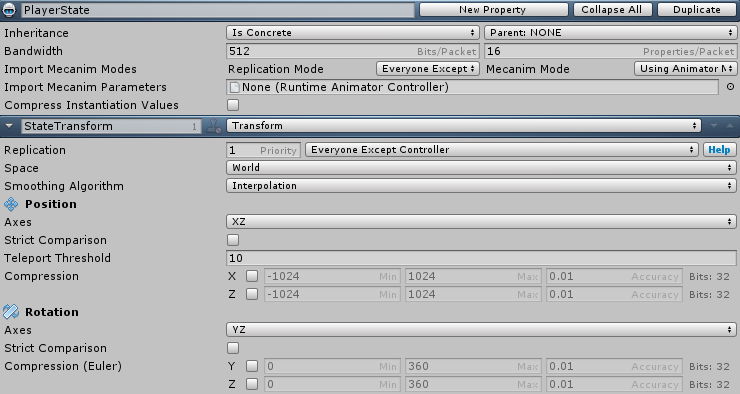
\includegraphics[scale=0.9]{statePacketOptimisation}
\end{center}

\newpage

\section{Potential Improvements}
\begin{itemize}
\item \textbf{Clicking "Join Random" in the lobby without any running sessions locks the client into an indefinite state} where they can't do anything and that they cannot escape without restarting the game. This is due to the bug described in the Lobby section that prevents the implementation of a check to verify the non existence of any sessions.
\item \textbf{While the player can name a session when creating one}, due to the above mentioned "BoltNetwork.Sessions" bug, no session list are displayed in the lobby and the name given by the player upon session creation \textbf{is not used} in any way.
\item Sessions cannot currently be protected by a password due to the "BoltNetwork.Sessions" bug.
\item In approaching the architecture of the program, I failed to consider the complexity that a multiplayer game implies. Therefore, while the \textbf{current architecture} gets the job done, it \textbf{would certainly benefit from some serious refactoring} to make it more granular, meaning to make the program very explicitly take into account that each player has their own worlds and that these need to be synchronized.
\end{itemize}

\section{Summary}
\textbf{The game fulfils it's basic ambitions}: \textbf{it is a barebone online FPS that successfully synchronizes players, performs hitscans for firing and triggers the appropriate gameplay feedbacks across the clients of all players.}\\\\
Photon Bolt has proven to be a difficult framework to work with. While it does provide some very useful features like the the synchronized hitboxes, it's transparency both in the code and in it's documentation makes debugging very difficult or even impossible like is the case with the "BoltNetwork.Sessions" list bug.\\
As a result, much of the time that has been allocated to this project was spent trying to solve unexplicable bugs or finding workarounds instead of expanding the features of the game, and some crucial features were outright impossible to implement.\\\\
\textbf{In conclusion, I am quite satisfied with the end result, as meagre it may appear.} During this project I've acquired the experience of working with a rather uncooperative framework, implementing the rather complex task of a responsive real-time online game, while tackling the problems encountered in a way to still provide a viable game at the end of the project.

\end{document}